\subsection{Image Modification}
An issue seen in LiDAR is the fact that object are often occluded, fragmented and do not appear with the same clarity as examples seen in satellite imagery. This means that we need to construct and train a network that is robust to changes in context and occlusion. Fortunately, research has been focussed in constructing better data augmentation techniques that attempt to solve those issues. Those techniques "mixes" different images from the dataset, covering parts of one another to make it harder for the network to correctly infer. CutMix\cite{cutMix} is one of those techniques. Mosaic, introduced by Bochkovsky, Wang and Liao in the YOLOv4 paper\cite{yolov4} creates a new images out of 4, by creating a "mosaic" of sort, where the 4 images can take varying portions of the new image. 


\subsection{Regularization and Normalization}
Regularization allows to reduce the complexity of a network and prevent overfitting. This is usually done by "dropping" random connections in a network, and training without those connections, a technique known as DropOut\cite{dropOut}. DropBlock\cite{dropBlock} relies on a similar method, but is more suitable for convolutional networks. DropBlock works by first choosing random seed points in a mask, and dropping a continuous region around those points. This is more effective than removing purely random activation as close activations contain closely related information.

\begin{figure}[H]
	\begin{subfigure}[t]{.3\textwidth}
  \centering
  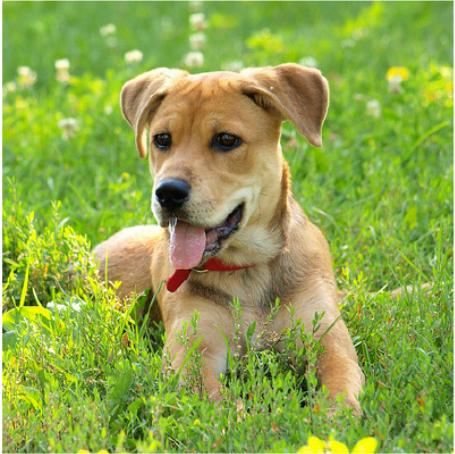
\includegraphics[width=.8\linewidth]{dogDropBlock}
  \caption{Base image}
  \label{fig:dropBlockA}
\end{subfigure}
	\begin{subfigure}[t]{.3\textwidth}
  \centering
  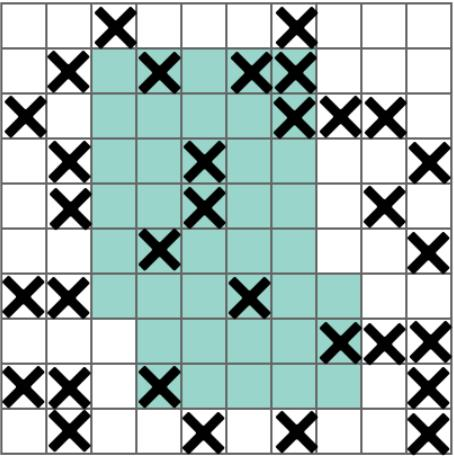
\includegraphics[width=.8\linewidth]{randomDrop}  
  \caption{Random Drop in activations}
  \label{fig:dropBlockB}
\end{subfigure}
	\begin{subfigure}[t]{.3\textwidth}
  \centering
  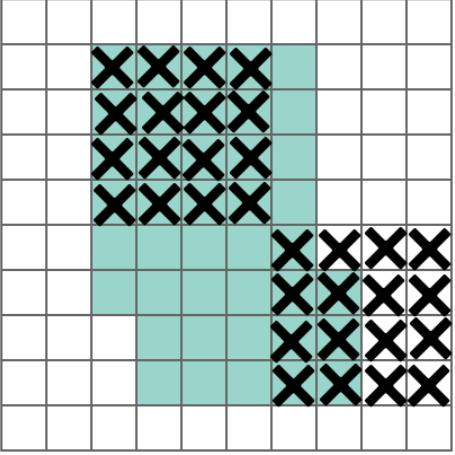
\includegraphics[width=.8\linewidth]{dropBlock}  
  \caption{DropBlock}
  \label{fig:dropBlockC}
\end{subfigure}
\caption{The blue regions represents neurons that contains semantic information on the base image. (b) shows the effect of removing activations at random, which is not effective as neurons close to each other contains closely related semantic information. (c) shows the DropBlock method, which have a better chance of entirely removing important semantic information on the base image, such as the head or the feet of the dog, forcing the remaining neurons to learn useful features}
\label{fig:dropBlock}
\end{figure}

Label smoothing~\cite{labelSmooth} convert hard labels, like one hot labeling into soft labels. This works by introducing a noise distribution in the labeling of the data, and converting the original label in relation to this noise distribution. \textbf{However, this label smoothing requires a rewriting of the loss system.}


